\subsection{Data Collector}
La componente \textit{data collector} permette di reperire i dati prodotti dai gateway che sono presenti all'interno dei vari topic di Kafka all'interno di un database di tipo timeseries. Allo stesso tempo permette di filtrare i messaggi che sono stati collezionati e inviare di conseguenza dei messaggi di avviso all'interno di un apposito topic.
Il filtraggio dei dati viene fatto degli alert impostati all'interno della web-app e salvati all'interno di un database relazionale (PostgreSql);
	\subsubsection{Diagramma dei package}%%%%%%%%%OK
	\begin{figure}[H]
			\centering
			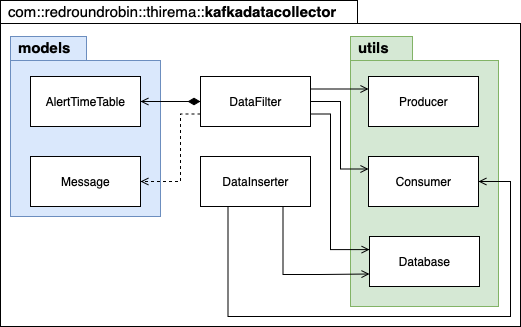
\includegraphics[scale=0.600]{res/images/DATACOLLECTOR/Packagekafkadatacollector.png}
			\caption{Diagramma dei package della componente Data Collector}
		\end{figure}
	\begin{landscape}
	\subsubsection{Diagramma delle classi}%%%%%%%%%%%%%%%%%%%%%%%OK
		\begin{figure}[H]
			\centering
			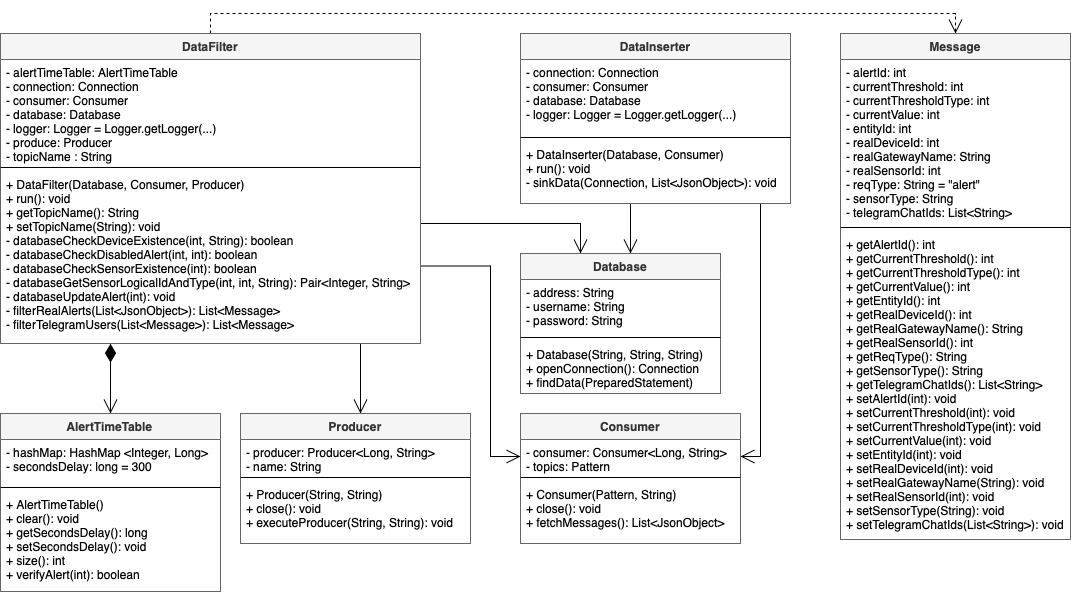
\includegraphics[scale=0.550]{res/images/DATACOLLECTOR/ClassikafkaDataCollector.png}
			\caption{Diagramma delle classi della componente Data Collector}
		\end{figure}
	\end{landscape}
	\begin{landscape}
	\subsubsection{Diagrammi di sequenza}
		\begin{figure}[H]
			\centering
			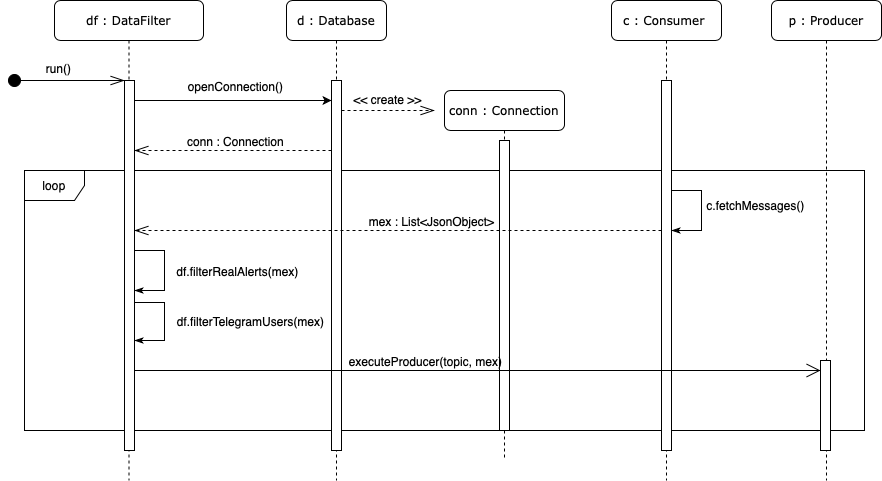
\includegraphics[scale=0.550]{res/images/DATACOLLECTOR/DataFilter.ThreadsKafkaDataCollector.png}
			\caption{Diagramma di sequenza in cui viene mostrato il funzionamento del filtraggio dati nella componente Data Collector}
		\end{figure}
		\begin{figure}[H]
			\centering
			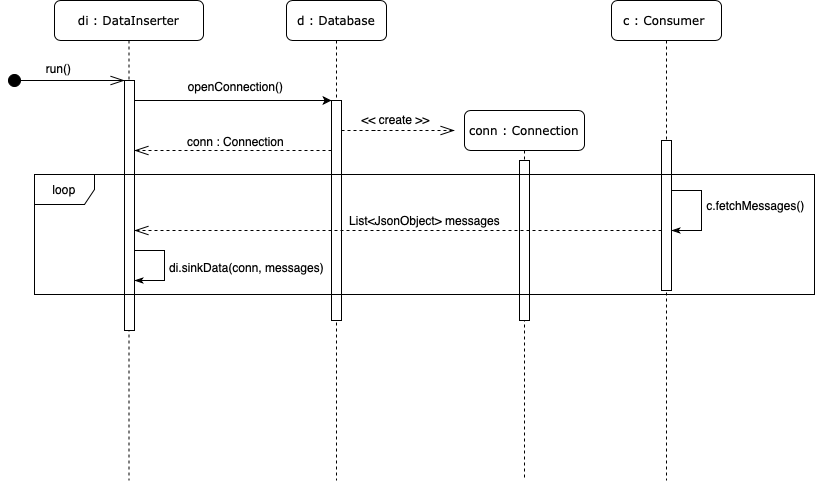
\includegraphics[scale=0.550]{res/images/DATACOLLECTOR/DataInserter.ThreadsKafkaDataCollector.png}
			\caption{Diagramma di sequenza in cui viene mostrato il funzionamento dell'inserimento dati nella componente Data Collector}
		\end{figure}
	\end{landscape}